\chapter{Particles in dual trees (pidt)}
\label{section:pidt}


\begin{figure}[htb]
 \begin{center}
  
\includegraphics[width=0.2\textwidth]{61_pidt/ExCALIBUR.png}
 \end{center}
 \caption{
   \Peano's particle handling is a follow-up to the 2015 paper ``Two
   Particle-in-Grid Realisations on Spacetrees''
   (\url{https://arxiv.org/abs/1508.02435}).
   Its full integration into \Peano\ has been made possible by the EPSRC grant 
   EP/V001523/1 (Massively Parallel Particle Hydrodynamics for Engineering and
   Astrophysics).
  }
\end{figure}


\subsection*{Preparing \Peano\ to run a particle code}

\Peano's particle code is lightweight and realised totally within the Python
API as \texttt{toolbox.particles}.
No particular configuration of the compute kernel is required.
To get something up and started, I recommend that you run the Jupyter notebook
at \texttt{examples/particles}.
It implements a very simple gravity $N$-body problem.


\section{Data model}

A particle in \Peano\ has at least two properties:

\begin{itemize}
  \item A position in space;
  \item A cut-off radius, i.e.~an environment of particles witch which it
  interacts.
\end{itemize}

\noindent
Particles are held on the heap, i.e.~you create them via \texttt{new} and then
you hand them over to \Peano\ to administer them.
Both properties can be changed dynamically by the user, i.e.~in each and every
time step.
Particles are to be modelled with \DaStGen.
You can think of them as plain C++ structs with a few routines to set their
properties and to send them around via MPI.


\section{Dual trees}

Particles are stored within the spacetree.
They are not necessarily stored on the finest mesh of the tree.

\begin{itemize}
  \item A particle resides on a mesh level within the tree such that the
  cut off radius $r \leq h$ if $h$ is the resolution of this level.
  \item A particle is associated to the vertex of this level that's closest to
  its centre $x$.
\end{itemize}

\noindent
These two conventions effectively span a dual grid over the spacetree if you
think of particles to be stored within cells.
\Peano\ automatically maintains these relations if you add the action set 
\texttt{peano4.toolbox.particles.UpdateParticleGridAssociation} to your
algorithmic steps.
As the convention relies on a smaller-equals sign, adaptive meshes are
automatically supported.
If particles travel through your domain and the mesh is not very fine, they
end up in the tree leaves.
If particles have a large cut-off radius, they are stored in rather coarse
levels of the tree.


If you change the cut-off radius or the position of a particle, the particle
will stay within its current cell/vertex within the tree.
In the next grid sweep, it will however we held by the ``correct'' vertex,
i.e.~its grid-vertex association will be updated.


If you add the action set
\texttt{peano4.toolbox.particles.PlotParticlesInVTKFormat} to your algorithm
step, the resulting file will contain all associativity information.
You can plot to which vertex a particle belongs to.


\paragraph{Example:}

\begin{center}
 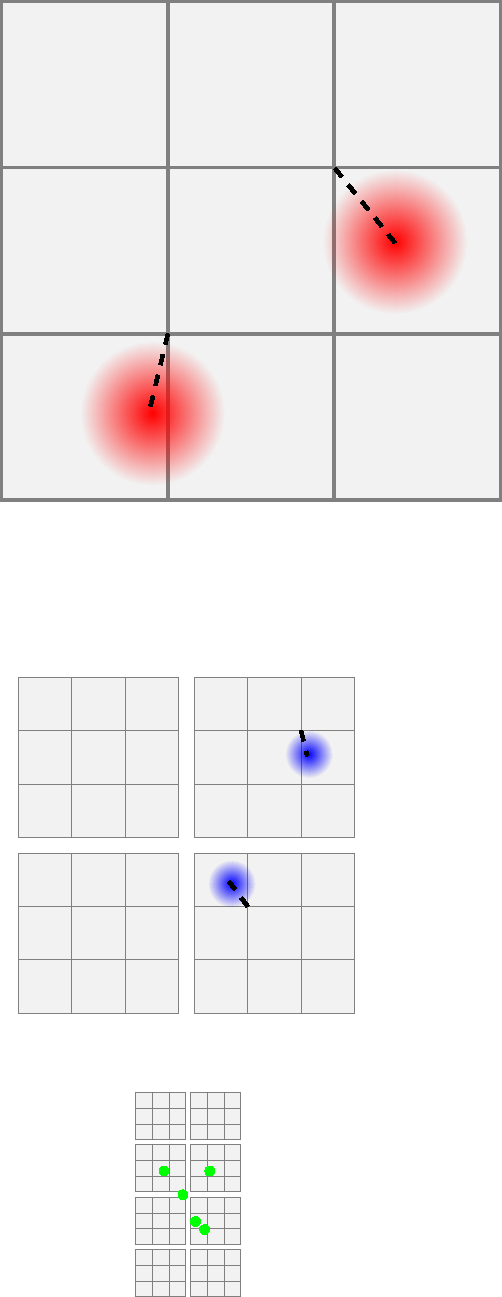
\includegraphics[width=0.25\textwidth]{61_pidt/dual-tree.pdf}
\end{center}

\noindent
A tree with three levels.
Particles with a large cut-off radius (red) are held on rather coarse levels.
Particles with very small cut-off are sorted (dropped) into the fine grid
levels.
Each particle is always associated to its closest vertex (dotted line).
It is the mesh which holds (owns) the vertices.
The toolset's predefined action set can automatically maintain/update these
associations after each grid sweep.
It also moves particles up and down the grid hierarchy if the particles' cut-off
radius changes or the grid changes.



\begin{definition}
  Our storage is vertex-oriented whereas most particle literature stores
  particles within cells.
  If we think of a dual multiscale mesh, i.e.~a mesh that is shifed by $h/2$
  alon each coordinate axis, then \Peano's approach also works with cells.
  Such shifted meshes are often called \emph{dual} meshes and I therefore speak
  of a \emph{dual tree}.
\end{definition}



\section{Particle-particle interaction}


\Peano\ always runs through the mesh top-down, i.e.~it traverses the spacetree
in a depth-first fashion.


Per cell, the code assembles a \texttt{local set}. 
This is a list of pointers to those particles that are associated to a cell's
$2^d$ vertices.
With the local set, you can make particles held on one resolution level
interact with each other.
You get an cubic area of $2h$ side-lenght per cell:
As a particle is always associated to its closest vertex, the local set holds all particles whose cut-off radius overlap with the cell. 


Adaptivity and particles with different cut-off are not yet captured through the
local set notion.
There's thus a second set that I call active set. 
The active set is the local set plus all local sets that have been active on
coarser levels within the tree.


If you use the \texttt{toolbox.particles.ParticleParticleInteraction} action
set, you pass it some C source code that works with the particles.
This C code has access to three variables: the active set, the local set and the
cell marker (of type \linebreak \texttt{peano4::datatraversal::CellMarker}).
Let's assume that each particle carries some velocity and that we could cut-off
gravity---which we clearly should not.


The straightforward particle-particle interaction then looks conceptionally as
follows:

\begin{code}
// Run over local set
for (auto& p: localParticles) {
  // Pick only those particles that reside within the current cell, otherwise
  // we would update each particle up to 2^d times. I do not exploit the
  // symmetry of forces here
  if ( marker.isContained( p->getX() ) ) {
    for (auto& pp: activeParticles) {
      // No interaction with particle itself
      if (p!=pp) {
        tarch::la::Vector<Dimensions,double> dist = pp->getX() - p->getX();
        [...]
      }
    }
  }
}
\end{code}




\section{Further action sets}

There are a few further action sets in the toolbox that help you to write your
Lagrangian code:


\begin{enumerate}
  \item The action set \texttt{toolbox.particles.UpdateParticleGridAssociation}
  is the core set. You'll always need this one to get the mapping of
  vertices/cells to particles right. The mapping is written in a way that it
  allows for \emph{tunnelling}, i.e.~particles may move more than one cell per
  grid sweep. In return, it is not necessary to update the particles in each and
  every time step---if your physics supports this.
  \item The action set \texttt{toolbox.particles.PlotParticlesInVTKFormat}
  provides a basic particle plotter which dumps particles, their cut-off radius
  plus their particle-vertex associativity. If you have to dump further
  properties, you have to write your own plotter. The generated plotter however
  can serve as a blueprint.
  \item The action set \texttt{toolbox.particles.ParticleTreeAnalysis} provides
  some fundamental tree analysis such as a multiscale counting how many
  particles reside within each cell. You'll need some additional data structures
  (per cell) to use this action set.
  \item The action set \texttt{toolbox.particles.ParticleAMR} uses the tree
  analysis to guide dynamic grid adaptivity. You can specify how many particles
  are held per cell at least, e.g., while the cut-off radius feeds naturally
  into the AMR.
\end{enumerate}


\section*{Links and further reading}

\begin{itemize}
  \item The ``official'' pidt paper is
{\tiny \begin{verbatim}
@article{WEINZIERL201642,
title = "Two particle-in-grid realisations on spacetrees",
journal = "Parallel Computing",
volume = "52",
pages = "42 - 64",
year = "2016",
issn = "0167-8191",
doi = "https://doi.org/10.1016/j.parco.2015.12.007",
url = "http://www.sciencedirect.com/science/article/pii/S0167819115001635",
author = "T. Weinzierl and B. Verleye and P. Henri and D. Roose",
keywords = "Particle-in-cell, Spacetree, Particle sorting, AMR, Lagrangian–Eulerian methods, Communication-avoiding"
}  \end{verbatim}}
  If you use the software, it would be great if you could cite this one.
\end{itemize}


